\subsection{Middlewares} 
Um \textit{middleware} comporta-se como uma ligação entre duas partes e permite executar código.

\begin{figure}[htb]
  \centering
  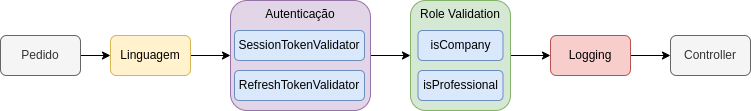
\includegraphics[width=\textwidth]{images/implementacao/api/middlewares.png}
  \caption{Comportamento de middlewares}
  \label{middlewares_png}
\end{figure}

\subsubsection{Linguagem}
O bem essencial para uma boa comunicação entre duas partes, é a utilização da mesma linguagem, pelo que, foi necessário perceber qual a linguagem a utilizar quando se responde a um pedido. Para este fim, foi desenvolvido um \textit{middleware}, cujo objetivo é verificar se existe a chave \textit{language} no cabeçalho do pedido. Caso esta exista, é obtida a linguagem e guardada nas variáveis locais do pedido. Na eventualidade desta não existir, a aplicação dará uma resposta em português por omissão. Este valor poderá ser futuramente alterado de forma simples.

\newpage

\subsubsection{Autenticação}
A autenticação dos utilizadores foi implementada através de \textit{JsonWebToken}. Este tipo de autenticação, tem por base a utilização de \textit{tokens} com tempo de expiração, o que significa que enquanto o \textit{token} estiver válido, o utilizador poderá realizar pedidos. Assim que o \textit{token} expirar, este terá de se autenticar novamente para obter um novo \textit{token}.
A utilização de \textit{tokens} permite assegurar que os pedidos são realizados com \textit{tokens}, gerados pela \textit{api}, através de uma chave de assinatura de \textit{token}, o que impede a utilização de \textit{tokens} gerados por utilizadores.
\begin{figure}[htb]
  \centering
  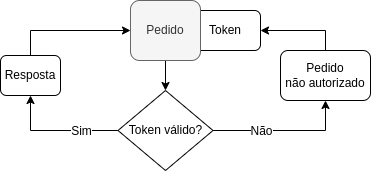
\includegraphics[width=0.5\textwidth]{images/implementacao/api/jwt_session.png}
  \caption{Utilização de tokens}
  \label{fig:64}
\end{figure}

A maior valência da utilização da técnica de autenticação mencionada anteriormente é a segurança. Isto acontece porque estes \textit{tokens} têm geralmente uma duração muito curta, como por exemplo, quinze minutos. Sempre que um \textit{token} de sessão expira o utilizador necessita realizar novamente o \textit{login}, o que poderá tornar a utilização da aplicação imprática.

A solução deste problema sem a perda de segurança significativa veio pelo meio da utilização de \textit{tokens} de duração maior em conjunto com os \textit{tokens} de duração curta. Enquanto o \textit{token} de grande duração se encontrar válido, novos \textit{tokens} de curta duração são gerados para o utilizador, o que leva a que o utilizador nunca perca a sua sessão. Estes \textit{tokens} de grande duração têm por nome \textit{refresh tokens} e os \textit{tokens} de curta duração têm por nome \textit{session tokens}. O utilizador sempre que termina a sessão o \textit{refresh tokens} deverá ser apagado.

Sempre que um utilizador realiza um pedido, o seu \textit{token} de sessão deverá ser validado. Caso este seja válido, o seu \textit{refresh token} deverá ser validado e apenas após esta verificação o utilizador estará autenticado. Na eventualidade de o \textit{token} de sessão ou de \textit{refresh} estiverem expirados, este estará sem autorização para realizar o pedido, mas, poderá solicitar um novo \textit{token} de sessão enquanto o seu \textit{refresh token} estiver válido. Isto acontece sem realizar novamente o \textit{login} e sem o utilizador perceber.

 Além das funcionalidades atrás mencionadas é possível também associar dados em formato \textit{json} a um \textit{token}. Esta funcionalidade foi utilizada para enviar o \textit{id} e o cargo do utilizador a qual pertence este \textit{token}.

 \newpage

\subsubsection{Validação de Papel}

Com a finalidade de garantir que apenas utilizadores com cargos suficientes conseguem realizar as ações regradas, foi desenvolvido um \textit{middleware} que valida se o utilizador que realizou o pedido tem permissões para o mesmo. Este \textit{middleware}, interliga-se com o \textit{middleware} anterior, pois, o cargo do utilizador em questão é enviado no \textit{token}, pelo que, é obtido e realizada uma comparação com o cargo desejado. Para isto foram criados dois \textit{middlewares} diferentes, um valida o cargo das empresas e o outro o cargo dos técnicos. As empresas podem realizar operações de técnicos, dado que, no \textit{middleware} de técnicos é verificado se o \textit{token} corresponde a um utilizador empresa, ou a um utilizador técnico. Já no \textit{middleware} de validação de empresa é verificado se o utilizador tem cargo de empresa.
